\chapter{EvoOracle: LLMs for Oracles}
\label{cha:evoOracles}
\vspace{0.4 cm}

In this chapter, we introduce EvoOracle, our innovative tool designed for efficient oracle generation using Large Language Models (LLMs). Figure 4.1 provides an insightful overview of EvoOracle's key components and workflow. To initiate the process, we acquire a dataset of Java open-source projects sourced from GitHub. Employing automated test case generation tools such as EvoSuite and Randoop, we systematically create Automated JUnit Test Cases for each project, laying the foundation for EvoOracle's subsequent operations. The tool begins by extracting metadata linked to the identified classes and methods within each project. Subsequently, it mines test cases and establishes mappings with corresponding focal methods extracted from the earlier project analysis. The SUT (System Under Test) Processor component plays a pivotal role in this phase, removing assertions from the test cases and substituting them with placeholders. Following this, the Prompt Processor component takes these test cases, now equipped with placeholders and focal methods, and formulates context for LLM prompting. The LLM Query Processor component utilizes this context to prompt the LLMs, passing the generated responses to the LLM Response Handler component. This handler, in turn, readies the test cases for execution. Finally, the Test Executor compiles and executes the newly generated tests, completing the comprehensive cycle of EvoOracle's oracle generation process.

\begin{figure}[H]
\centering
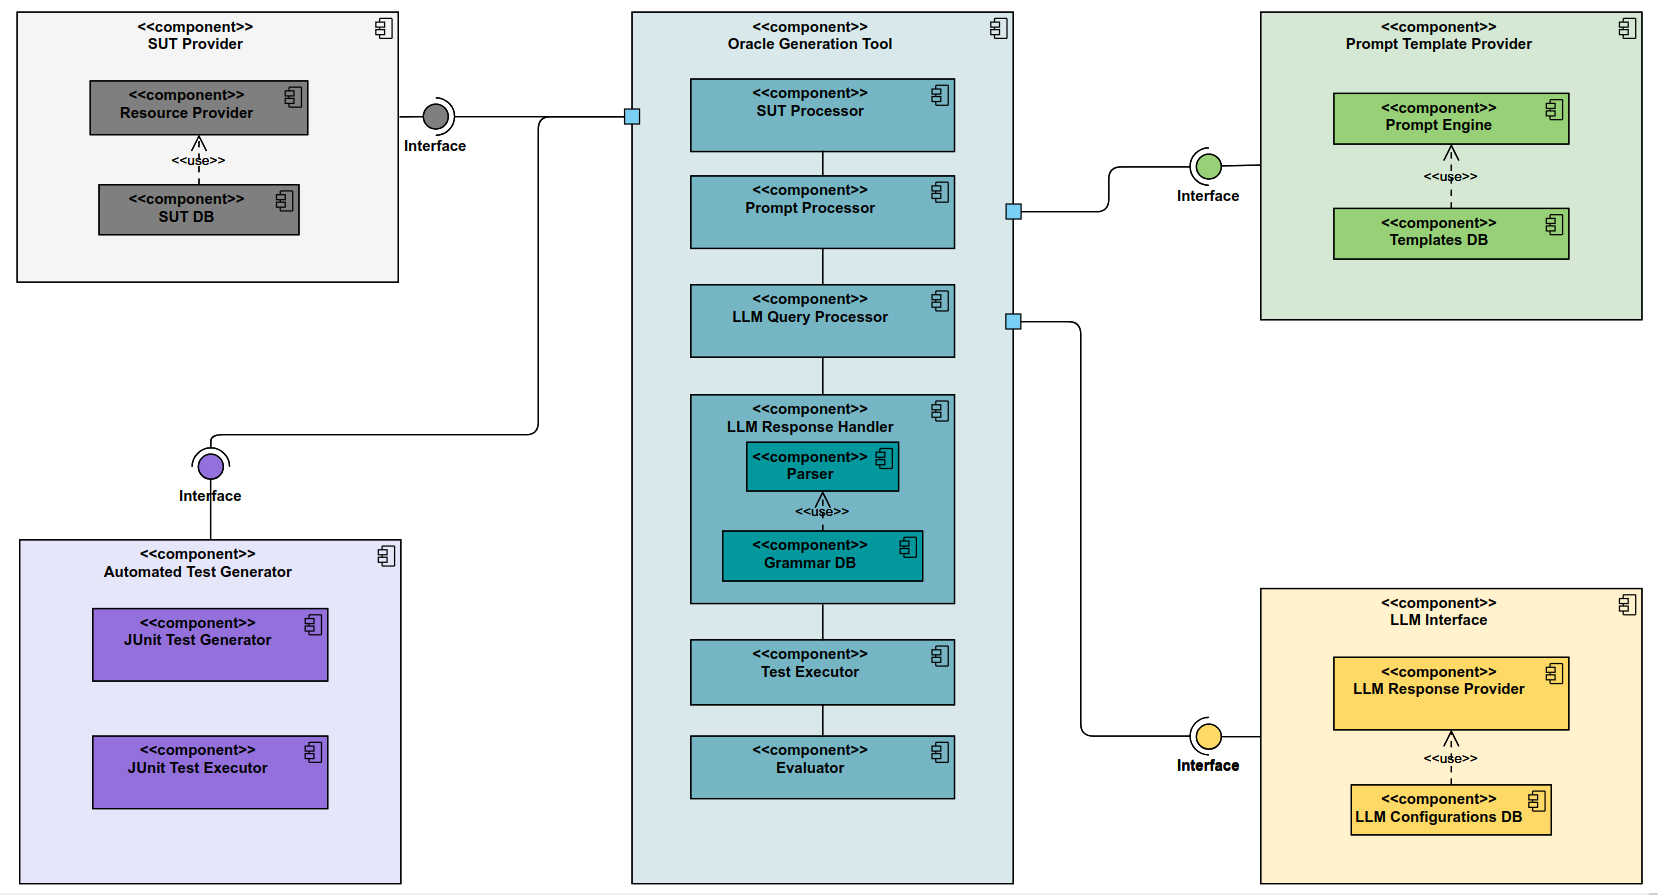
\includegraphics[width=1\textwidth]{images/UML_Component_Diagram_EvoOracle_v2.png}
\caption{Components of our proposed tool: EvoOracle}
\label{fig:component_diagram}
\end{figure}

In the following sub-chapters, we will delve into the intricacies of each step, providing detailed descriptions and insights into the nuances of EvoOracle's comprehensive process.

\section{Data Collection}
\label{sec:data_collection}
\vspace{0.2 cm}
Within this sub-chapter, we will elaborate on our methodology for assembling a collection of Java projects. We outline the procedures involved in generating test cases using automated tools such as EvoSuite and Randoop, shedding light on the meticulous steps taken to ensure comprehensive test coverage. Additionally, we will discuss the meticulous process of preparing corresponding focal methods, elucidating how we identify and associate the specific methods targeted by each test case. This step is crucial in establishing a robust foundation for subsequent analyses and evaluations within the realm of software testing and development.

\vspace{0.1 cm}
\subsection{Java Projects Selection}
\label{sec:projects_selection}
\vspace{0.1 cm}

We select 4 projects as shown in Table \ref{tab:collected_java_projects} of all the public GitHub Java repositories declaring an open source license, which have been updated within the last three years, and has the most stars or forks. We also considered recent projects to avoid possible Data Leakage and tried to choose project as diverse as possible from each other to make sure our tool is exposed to diverse projects. From these 4 projects and a total of 388 classes, we randomly chose 9 classes. The details about these classes are shown in Table \ref{tab:selected_java_projects}.

\begin{table}
    \centering
    \begin{tabular}{l | l | r}
        \textbf{Project Name} & \textbf{Classes} & \textbf{Reference} \\
        \hline
        frontend-maven-plugin & 43 & \cite{sletteberg_frontend-maven-plugin_2023} \\
        javacv & 117 & \cite{noauthor_bytedecojavacv_nodate} \\
        webdrivermanager & 44 & \cite{noauthor_bonigarciawebdrivermanager_nodate} \\
        zerocode & 184 & \cite{noauthor_authorjappszerocode_nodate} \\
    \end{tabular}
\caption{Details of the collected Java projects.}
\label{tab:collected_java_projects}
\end{table}

\begin{table}
    \centering    
    \begin{tabular}{l | l | r}
        \textbf{Class Name} & \textbf{Project Name} & \textbf{Methods} \\
        \hline
        BaseSettings & javacv & 6 \\
        Parallel & javacv & 6 \\
        SeekableByteArrayOutputStream & javacv & 3 \\
        NPMInstaller & frontend-maven-plugin & 15 \\
        NodeInstaller & frontend-maven-plugin & 18 \\
        PnpmInstaller & frontend-maven-plugin & 14 \\
        CacheHandler & webdrivermanager & 4 \\
        PropertiesProviderUtils & zerocode & 4 \\
        ZerocodeCorrelationshipLogger & zerocode & 17 \\
    \end{tabular}
\caption{Summary of selected Java projects.}
\label{tab:selected_java_projects}
\end{table}

\vspace{0.1 cm}
\subsection{Test Case Generation with EvoSuite}
\label{sec:test_case_generation}
\vspace{0.1 cm}

In this subsection, an overview of ...

\vspace{0.1 cm}
\subsection{Data Extraction (Class, Method, Dependencies, etc.)}
\label{sec:data_extraction}
\vspace{0.1 cm}

First, we parse each project to obtain classes and methods with their associated metadata. Next, we identify each test class and its corresponding focal class. Finally, for each test case within a test class, we map it to the related focal method obtaining a set of mapped test cases.


\section{Preprocessing}
\label{sec:preprocessing}
\vspace{0.2 cm}

In this section, ...

\vspace{0.1 cm}
\subsection{Removal of Assertions from Test Cases}
\label{sec:assertion_removal}
\vspace{0.1 cm}

In this subsection, an overview of ...

\vspace{0.1 cm}
\subsection{Placeholder Insertion}
\label{sec:placeholder_insertion}
\vspace{0.1 cm}

In this subsection, ...

\section{Large Language Model Integration}
\label{sec:llm_integration}
\vspace{0.2 cm}

In this section, ...

\vspace{0.1 cm}
\subsection{LLM Selection and Configuration}
\label{sec:llm_configurations}
\vspace{0.1 cm}

In this subsection, an overview of ...

\vspace{0.1 cm}
\subsection{Prompt Preparation}
\label{sec:prompt_preparation}
\vspace{0.1 cm}

In this subsection, ...

\vspace{0.1 cm}
\subsection{Generating Assertions}
\label{sec:generating_assertions}
\vspace{0.1 cm}

In this subsection, ...

\vspace{0.1 cm}
\subsection{Evaluating Response Quality}
\label{sec:evaluating_response}
\vspace{0.1 cm}

In this subsection, ...

\section{Test Case Preparation}
\label{sec:test_case_preparation}
\vspace{0.2 cm}

In this section, ...

\vspace{0.1 cm}
\subsection{Assertion Integration}
\label{sec:assertion_integration}
\vspace{0.1 cm}

In this subsection, ...

\vspace{0.1 cm}
\subsection{Test Case Compilation}
\label{sec:test_compilation}
\vspace{0.1 cm}

In this subsection, an overview of ...